% ==========================================================================
% Metodologia, implementación y resultados
% ==========================================================================

\section{Metodología}\label{sec:metodologia}

Para evaluar el desempeño de las estrategias de despacho se desarrolló un simulador
en MATLAB que replica de forma conceptual el proceso de
despacho en enlace descendente de una celda celular basada en 4G/5G.
El simulador implementa cuatro estrategias de despacho: Round Robin (RR), 
Best CQI (BCQI), Blind Equal Throughput (BET) y Proportional Fair (PF). 
Las cuatro comparten el mismo modelo de red, canal y tráfico. La diferencia
entre ellas es la forma con la que se decide el orden y prioridad en el que 
se les asignan bloques de recurso (RB) a los equipo de usuario (UE) conectados
a la red. En esta sección se describe el modelo de asignación de recursos
y la implementación de cada despachador.

La estructura de recursos del simulador se basa en LTE-A, la cual
comparte con 5G su numerología base ($\mu = 0$) el espaciado entre
subportadoras de 15~kHz, los RB de 12 subportadoras y la trama de 10~ms
\citep{lin2019}.

\subsection{Modelo de red y de canal}\label{subsec:modelo}

Se considera una celda con una radiobase (gNB) ubicada en el centro y $N$
UE distribuidos dentro de un radio $r$. Al inicio de cada simulación, los
UE se distribuyen a lo largo de la gNB y el borde de la celda. Se
mantiene la misma distancia entre UEs.
\begin{equation}
  d_i = r\,\frac{i-1}{N-1}, \qquad i = 1, \dots, N,
  \label{eq:distancias}
\end{equation}

La potencia recibida por el UE $i$ se obtiene como
$P_{rx,i} = P_{tx} - PL(d_i)$, donde $P_{tx}$ es la potencia de
transmisión de la gNB en dBm y $PL(d_i)$ son las pérdidas por
propagación del modelo Urban Macro sin línea de vista (UMa NLOS)
\textbf{[3GPP TR~38.901]}.

La relación señal a ruido más interferencia del UE $i$ en el RB $k$ se
calcula en dB como
\begin{equation}
  \gamma_{i,k} = P_{rx,i} - \left(-174 + 10\log_{10}B\right) - I_{i,k},
  \label{eq:sinr}
\end{equation}
donde $B$ es el ancho de banda del canal en Hz y $I_{i,k}$ es una variable
aleatoria en dB que representa la degradación de la señal por
interferencia. Este valor se obtiene como el absoluto de una
variable aleatoria normal con media cero y desviación estándar
$\sigma_I = N f_I$, donde $f_I$ es un factor de interferencia por usuario.
De esta forma, la interferencia crece con el número de UE en la celda. El
valor de $\gamma_{i,k}$ se genera de nuevo para cada UE, en cada RB y en
cada trama.

Para la adaptación del enlace, $\gamma_{i,k}$ se compara con un conjunto
de umbrales para obtener el índice de CQI (de 1 a 15) de la tabla de 4
bits de 3GPP TS 36.213 \textbf{[CITA REQUERIDA]}. Con
$\gamma_{i,k}$ se obtiene el CQI, que determina los bits que transporta el RB.

El despacho se realiza por trama (10 ms). El número de RB disponibles en
una trama es $K = 20\,N_{RB}$, donde $N_{RB} = 5B$ (con $B$ en MHz) es el
número de RB por ranura de 0.5~ms y 20 es el número de ranuras en una
trama. Los RB de la trama se asignan uno a la vez, y cada RB se asigna a un
solo UE.

En cuanto al tráfico, se considera un modelo de buffer infinito: todos los
UE tienen siempre datos por recibir y permanecen en la celda durante toda
la simulación, por lo que el número de UE activos se mantiene igual a $N$.
La simulación termina después de $F$ tramas.

\subsection{Implementación}\label{subsec:implementacion}

La Fig.~\ref{fig:flujo} muestra el proceso de despacho de los
cuatro despachadores presentados. Al inicio de cada trama se calcula
$\gamma_{i,k}$ para todos los UE y todos los RB de la trama. Después, para
cada RB $k$, el despachador calcula la métrica $m_{i,k}$ de cada UE activo
y asigna el RB al UE con la métrica más alta,
\begin{equation}
  i^{*} = \arg\max_{i \in \mathcal{A}} \; m_{i,k},
  \label{eq:argmax}
\end{equation}
donde $\mathcal{A}$ es el conjunto de UE que aún tienen datos por recibir.
Al terminar la trama se registran los datos entregados a cada UE
y el proceso se repite hasta completar las $F$ tramas. 
Después de completar todas las tramas, se calculan las métricas de
desempeño de los algoritmos de despacho.

\begin{figure}[tb]
\centering
\begin{tikzpicture}[
    font=\scriptsize,
    node distance=3.2mm,
    proc/.style={rectangle, draw, align=center, text width=40mm,
                 minimum height=5mm, inner sep=1.5pt},
    term/.style={rectangle, draw, rounded corners=2.5mm, align=center,
                 text width=28mm, minimum height=5mm},
    dec/.style={diamond, draw, aspect=2.6, align=center, inner sep=0.5pt},
    flecha/.style={-{Latex[length=1.6mm]}}
  ]
  \node[term] (ini) {Inicio};
  \node[proc, below=of ini] (par)
    {Definir parámetros y ubicar $N$ UE con (\ref{eq:distancias})};
  \node[proc, below=of par] (snr)
    {Nueva trama: calcular $\gamma_{i,k}$ para todo UE y RB con (\ref{eq:sinr})};
  \node[proc, below=of snr] (met)
    {Calcular $m_{i,k}$ de cada UE activo según el despachador};
  \node[proc, below=of met] (asig)
    {Asignar el RB $k$ al UE $i^{*}$ con (\ref{eq:argmax})};
  \node[proc, below=of asig] (bits)
    {Obtener CQI y sumar los bits del RB a los datos del UE $i^{*}$};
  \node[dec, below=of bits] (finrb) {¿Último RB\\de la trama?};
  \node[dec, below=of finrb] (fintr) {¿Trama $F$?};
  \node[proc, below=of fintr] (metr) {Calcular métricas de desempeño};
  \node[term, below=of metr] (fin) {Fin};

  % Coordenadas de los lazos, a la izquierda de los bloques
  \coordinate (xk) at ($(met.west)+(-3mm,0)$);
  \coordinate (xf) at ($(met.west)+(-6mm,0)$);

  \draw[flecha] (ini) -- (par);
  \draw[flecha] (par) -- (snr);
  \draw[flecha] (snr) -- (met);
  \draw[flecha] (met) -- (asig);
  \draw[flecha] (asig) -- (bits);
  \draw[flecha] (bits) -- (finrb);
  \draw[flecha] (finrb.west) -- node[above] {No} (finrb.west -| xk)
     -- node[midway, sloped, above, inner sep=1pt] {$k \leftarrow k+1$} (xk)
     -- (met.west);
  \draw[flecha] (finrb) -- node[right] {Sí} (fintr);
  \draw[flecha] (fintr.west) -- node[above] {No} (fintr.west -| xf)
     -- (snr.west -| xf) -- (snr.west);
  \draw[flecha] (fintr) -- node[right] {Sí} (metr);
  \draw[flecha] (metr) -- (fin);
\end{tikzpicture}
\caption{Diagrama de flujo del proceso de despacho de los
  despachadores RR, BCQI, BET y PF.}
\label{fig:flujo}
\end{figure}

\subsubsection{Round Robin (RR).}
RR asigna los RB a los UE por turnos, en un orden fijo y sin
considerar las condiciones del canal ni los requerimientos del
usuario \citep{capozzi2013,fitriasari2021}. Su métrica se puede expresar como
\begin{equation}
  m^{RR}_{i,k} = t - T_i,
  \label{eq:rr}
\end{equation}
donde $t$ es el tiempo actual y $T_i$ es la última vez que el UE $i$ fue
atendido \citep{capozzi2013}, de manera que se prioriza al UE que lleva
más tiempo sin que se le asignen recursos. Con esta estrategia todos los UE
reciben la misma cantidad de RB.

\subsubsection{Best CQI (BCQI).}
BCQI asigna cada RB al UE que puede alcanzar la mayor tasa de datos en ese RB,
con el objetivo de maximizar el throughput del sistema sin importar la equidad
\citep{capozzi2013,haque2023}. En la implementación, la métrica es el
SINR del UE en el RB,
\begin{equation}
  m^{BCQI}_{i,k} = \gamma_{i,k}.
  \label{eq:bcqi}
\end{equation}
Debido a que el CQI y, por lo tanto, la cantidad de bits que puede transportar
el RB no disminuyen al aumentar $\gamma_{i,k}$, elegir el UE con mayor SINR 
equivale a elegir el UE que transporta más bits en el RB. Los UE cercanos 
a la gNB son atendidos con mayor frecuencia, mientras que los UE 
en el borde de la celda pueden no ser atendidos hasta que mejoren sus 
condiciones de canal.

\subsubsection{Blind Equal Throughput (BET).}
BET busca la equidad en términos de throughput, para lo cual prioriza al
UE que ha recibido menos datos, sin considerar las condiciones del
canal \citep{capozzi2013}. La métrica de BET es
\begin{equation}
  m^{BET}_{i,k} = \frac{1}{\bar{R}_i(k-1)},
  \label{eq:bet}
\end{equation}
donde $\bar{R}_i$ es el promedio de datos recibidos del UE $i$
\citep{capozzi2013}. En la implementación, $\bar{R}_i$ se actualiza en cada
RB. Los UE que todavía no han sido atendidos tienen $\bar{R}_i = 0$ y,
por lo tanto, la métrica más alta, por lo que se atienden primero.

\subsubsection{Proportional Fair (PF).}
PF busca un punto medio entre BCQI y BET: favorece a los UE con buenas
condiciones de canal, pero tomando en cuenta el throughput que cada UE ha
recibido \citep{capozzi2013,fitriasari2021}. Su métrica es
\begin{equation}
  m^{PF}_{i,k} = \frac{r_{i,k}}{\bar{R}_i(k-1)},
  \label{eq:pf}
\end{equation}
donde $r_{i,k}$ es la tasa que alcanzaría el UE $i$ en el RB $k$ y
$\bar{R}_i$ es su throughput promedio \citep{capozzi2013}.
Un UE con buenas condiciones de canal tiene un numerador
alto, pero su métrica disminuye conforme aumenta su throughput, lo que
permite que los UE con peores condiciones sean atendidos cuando su
throughput promedio es bajo.

\subsection{Métricas de desempeño}\label{subsec:metricas}

Al final de cada simulación se calculan las siguientes métricas:

\begin{itemize}
  \item Throughput de la celda: total de bits entregados a todos los UE
    entre el tiempo simulado.
  \item Eficiencia espectral: throughput de la celda dividido entre el
    ancho de banda del canal, en bits/s/Hz. Indica qué tan bien se
    aprovecha el espectro disponible \citep{mamane2022}.
  \item Equidad: índice de Jain sobre el throughput de cada UE,
    \begin{equation}
      J = \frac{\left(\sum_{i} x_i\right)^2}{n \sum_{i} x_i^2},
      \label{eq:jain}
    \end{equation}
    donde $x_i$ es el throughput del UE $i$, es decir, la cantidad de
    datos que recibió dividida entre el tiempo simulado, y $n = N$ es el
    número de UE \citep{shi2014}.
\end{itemize}
\subsection{Resultados}\label{sec:resultados}

Los cuatro despachadores se evaluaron en la misma celda y bajo las mismas
condiciones, según la tabla~\ref{tab:parametros}.

Con buffer infinito, todos los UE permanecen en la celda durante toda la
simulación. Lo anterior permite observar cómo asigna cada despachador los
recursos sin modificar sus condiciones de paquete de datos. Cada
despachador se simula durante 1~s y cada simulación inicia con la misma 
generación de números aleatorios.

\begin{table}[tb]
\centering
\caption{Parámetros de simulación.}
\label{tab:parametros}
\footnotesize
\begin{tabular}{ll}
\hline
Parámetro & Valor \\
\hline
UE activos ($N$) & 40 \\
Radio de la celda ($r$) & 1~km \\
Frecuencia portadora & 2.6~GHz \\
Potencia de transmisión ($P_{tx}$) & 43~dBm \\
Ancho de banda del canal ($B$) & 5~MHz \\
Modelo de pérdidas & UMa NLOS \\
Factor de interferencia ($f_I$) & 0.1 \\
Duración ($F$) & 100 tramas (1~s) \\
Tráfico & Buffer infinito \\
\hline
\end{tabular}
\end{table}

\subsubsection{Throughput por UE.}\label{subsec:res_tp}

La fig.~\ref{fig:tp} muestra el throughput promedio de cada UE en función
de su distancia a la gNB. Con RR, cada UE recibe
el 2.5\% de los RB disponibles, por lo que su throughput depende solo de
las condiciones del canal.

BCQI asigna cada RB al UE con mayor SINR, de modo que solo atiende a los
dos UE más cercanos: el UE ubicado junto a la gNB recibe el 93.8\%
de los RB (21.9~Mbps) y el UE a 25.6~m el resto (1.4~Mbps). Los 38 UE
restantes no reciben datos y no aparecen en la figura.

BET iguala el throughput de todos los UE. Para lograrlo, asigna más RB 
a los UE con peores condiciones de canal (del 1.6\% para el UE más
cercano al 5.3\% para el UE del borde), lo que reduce el throughput de los
UE que se encuentran más cerca del gNB con respecto a RR y PF.

PF reparte los RB casi en la misma proporción que RR (entre 2.42\% y
2.50\% por UE), pero a cada UE se le asignan los RB en los que tiene menor
interferencia.

\begin{figure}[tb]
\centering
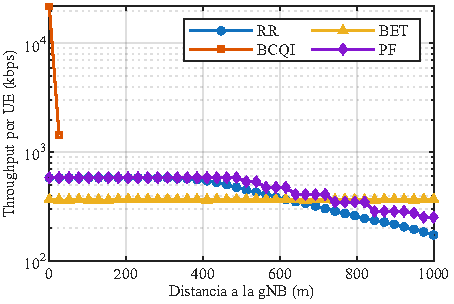
\includegraphics[width=\columnwidth]{figuras/fig_tp_distancia.pdf}
\caption{Throughput por UE en función de la distancia a la
  gNB. Los 38 UE sin servicio con BCQI tienen throughput 0 y no
  se muestran en la gráfica.}
\label{fig:tp}
\end{figure}

La Tabla~\ref{tab:metricas} resume las métricas calculadas en la simulación.
BCQI obtiene el mayor throughput de la celda (23.3~Mbps, que
equivale a una eficiencia espectral de 4.67~bits/s/Hz), pero con un valor de
equidad según el índice de Jain de 0.03. BET alcanza una equidad 
prácticamente perfecta ($J = 1.00$) con el menor throughput (14.6~Mbps).
PF obtiene el segundo mayor throughput (19.1~Mbps, 11\% más que RR) y una 
equidad de 0.94, mayor que la de RR (0.89).

\begin{table}[tb]
\centering
\caption{Métricas globales por despachador.}
\label{tab:metricas}
\footnotesize
\begin{tabular}{lccc}
\hline
Despachador & Throughput & Eficiencia espectral & $J$ \\
 & (Mbps) & (bits/s/Hz) & \\
\hline
RR   & 17.2 & 3.44 & 0.89 \\
BCQI & 23.3 & 4.67 & 0.03 \\
BET  & 14.6 & 2.93 & 1.00 \\
PF   & 19.1 & 3.83 & 0.94 \\
\hline
\end{tabular}
\end{table}

Los resultados muestran el compromiso entre throughput y equidad de cada
estrategia de despacho. BCQI maximiza el throughput de la celda a cambio de dejar sin
servicio a una gran cantidad de UE, mientras BET logra la mayor equidad a cambio
de menor throughput y otorgar menos recursos a los UE cercanos al gNB.
RR reparte los recursos por igual, pero no aprovecha las condiciones del
canal para asignar recursos. PF ofrece el mejor balance: el segundo mayor throughput de la
celda, una equidad de 0.94 y 45\% más throughput que RR para el UE que se encuentra
en el borde de la celda.
